\chapter{Directed Nearest Neighbor}
\label{cha:directed_nearest_neighbor}
To improve the Nearest Neighbor algorithm we now not only search for the nearest neighbor but also look at the direction we are going while constructing the curve. In this way not always the nearest neighbor of a certain point is chosen, but a point which differs the least in direction from the previous edge from all other points within a certain range.

  \section{Lexicographic Smallest}
  \label{sec:lexicographic_smallest}
    LexicographicSmallest was not changed for DirectedNearestNeigbor, for analysis of this function see \ref{ref:ls}.

  \section{Find Points In Range}
  \label{sec:find_points_in_range}

    \subsection{Definitions}
    \label{sub:definitions}
      \begin{definition} \label{def:fpir}
          Given the range $\alpha$, the point from which to look, $p$, and the set of points which still need to be processed, $S$, FindPointsInRange returns all points in $S$ that lie within range $\alpha$ from $p$.
      \end{definition}
      
    \subsection{Functional Description}
    \label{sub:functional_description}
      This function finds all points which lie in a certain range.\\
      We give this function three parameters: one for the range, one for a point, $p$, and one for the array $S$ with all the points that we want to be checked. In the function we make an array $R$ which we will use to store all points in the range.\\
      Now we compare, for all points in $S$, the distance between $p$ and a point in $S$, say $x$, to the range. If the distance is smaller than the range we will store $x$ in $R$.\\
      When all points in $S$ are used in the comparisons $S$ is returned.

    \subsubsection{Proof of correctness}
    \label{ssub:proof}
      Assume $q$ is a point that lies outside range $\alpha$ from $p$ and is returned by FindPointsInRange.\\
      According to the if-statement in FindPointsInRange in which is checked whether or not a point lies within range $\alpha$ from $p$ or not, so $q$ cannot be part of the set of points which lie in range $\alpha$.\\
      This is in contradiction to the assumption.\\
      So FindPointsInRange returns only those points that lie in range $\alpha$ from $p$.

    \subsection{Running Time Analysis}
    \label{sub:running_time_analysis}
      This function consists of a single for loop that goes through all of its inputs elements. In the for loop is a single if statement, that checks the distance between the given point and the current point. If the current point is within the given range, it is added to the solution. \\
      This takes $O(n)$ time.

  \section{Give Best Point}
  \label{sec:give_best_point}

    \subsection{Definitions}
    \label{sub:definitions}
      \begin{definition} \label{def:gbp}
          Given the edge $(p,q)$ and the set $S$, with $S$ being the $n$ points within range $\alpha$ from $q$, GiveBestPoint returns the best point $r$ in $S$, if the angle of the edge $(q,r)$ differs the least from the angle of the preceding edge $(p,q)$.\\ (All angles are with respect to the x-axis).
      \end{definition}
      \emph{Note:} This definition does not hold for connecting the first two points, this is done by using NearestNeighbor.

    \subsection{Functional Description}
    \label{sub:functional_description}
      We have one array $S$.\\
      We will call the first point in the array $p$, the second $q$, and the rest $1,2,3..Count-2$.\\
      We first calculate the angle of the edge between $p$ and $q$ called $a$.\\
      Next we calculate the angle between $q$ and $1$, we compare this angle to $z$ and store point $1$ as the best point so far.\\
      We now do the same for all the points left in array $S$ and if the comparison of a new angle is smaller then the one we had so far, we store the point which makes the edge with $q$ as the best so far.\\
      When all points in $S$ have been checked we return the stored point which should now have the smallest angle in comparison to $z$.


    \subsubsection{Proof of correctness}
    \label{ssub:proof}
      GiveBestPoint starts with computing the angle of edge $(p,q)$, then it calculates the angle of the edges between $q$ and one of the $n$ points in $S$ and compares it to the angle of edge $(p,q)$. This is done for all $n$ points, while keeping track of the best point so far, say $r$.\\
      So after all edges are processed $r$ is returned, which is indeed the point which angle differs the least from the angle of edge $(p,q)$.

    \subsection{Running Time Analysis}
    \label{sub:running_time_analysis}
      This function consists of a single loop that goes through all of its inputs elements, and several if statements. GiveBestPoints first calculates the angle of it's first line segment than goes into the for loop. The for loop goes through all other points, makes the line segment, calculates the angle and compares it with the current best (and replaces if so). After the for loop it returns the solution. \\
      Because only the for loop takes longer than constant time, the running time of GiveBestPoint is $O(n)$

  \section{Directed Nearest Neighbor}
  \label{sec:directed_nearest_neighbor}

    \subsection{Definitions}
    \label{sub:definitions}
      \begin{definition}
          Given a set $S$ of $n$ input points, DirectedNearestNeighbor returns the curve with the least change of direction.
      \end{definition}

    \subsection{Functional Description}
    \label{sub:functional_description}
      
      \begin{figure}
        
        \begin{tabular}{lr}
       \textbf{DirectedNearestNeighbor}$(P)$                                & \\
        $ls,p \gets $ \textbf{LexicograhicSmallest}$(P),P[ls]$              & \\
        \textbf{for} $i \gets 0$ \textbf{to} $|P| - 2$ \textbf{do}          & \\
        \qquad $P,skip \gets P \backslash \{ p\},false$                     & \\
        \qquad \textbf{if} $|A| \geq 2$ \textbf{then}                       & \\
        \qquad \qquad $skip \gets true$                                     & \\
        \qquad \qquad $r \gets \alpha * d(A[|A|-1],A.last) $                & \\
        \qquad \qquad $B \gets $ \textbf{FindPointsInRange}$(P,p,r)$        & \\
        \qquad \qquad \textbf{if} $|B| = 0$ \textbf{then}                   & \\
        \qquad \qquad \qquad $skip \gets false$                             & \\
        \qquad \qquad \textbf{elseif} $|B| = 1$ \textbf{then}               & \\
        \qquad \qquad \qquad $q \gets B[0]$                                 & \\
        \qquad \qquad \textbf{else}                                         &\\
        \qquad \qquad \qquad $B \gets \{A.last\} \cap \{A[|A|-1]\} \cup B$  & \\
        \qquad \qquad \qquad $q \gets$ \textbf{GiveBestPoint}$(P)$          &  \\
        \qquad \qquad \textbf{fi}                                           & \\
        \qquad \textbf{fi}                                                  & \\
        \qquad \textbf{if} \textbf{not} $skip$ \textbf{then}                & \\
        \qquad \qquad $r,q \gets \infty,p$                                  & \\
        \qquad \qquad \textbf{for} $j \gets 0$ \textbf{to} $|P| - 1$ \textbf{do}  & \\
        \qquad \qquad \qquad $c \gets d(p,P[J])$                            & \\
        \qquad \qquad \qquad \textbf{if} $c < r$ \textbf{then}              & \\
        \qquad \qquad \qquad \qquad  $r,q \gets c, P[j]$                    & \\
        \qquad \qquad \qquad \textbf{fi}                                    & \\
        \qquad \qquad \textbf{od}                                           & \\
        \qquad \textbf{fi}                                                  & \\
        \qquad $A,p \gets A \cup {q},q$                                     & \\
       \textbf{od}                                                          & \\ \hline
        \qquad \qquad \qquad\qquad\qquad\qquad\qquad \textbf{Total }        & $O(n^{2})$ 
        \end{tabular}
        
        \label{fig:dnncode}
        \caption{The pseudocode for DirectedNearest Neighbor}
      \end{figure}
      
      We augmented NearestNeighbor (\ref{ref:nn}).\\
      We now use one more array $C$ which is initially empty.\\
      Finding the first and second point of the solution stays the same. When we have those two points we calculate a range. The range is the distance between the last two points multiplied by a constant $c$.\\
      Now we use the subfunction FindPointsInRange (\ref{ref:fpir}). We give three parameters: the range, the last point in our solution and the array $A$. We store the result of FindPointsInRange in $C$. We now insert the last point, and the second last point of $B$ into $C$ (Make sure that those points are the first two in $C$).\\
      If there are less than two points in the result of FindPointInRange we just take the Nearest Neighbor.\\
      If there two points or more we call subfunction GiveBestPoint (\ref{ref:gbp}). As parameter we give array $C$. We now add the result of GiveBestPoint to $B$ and delete the result from $A$.\\
      These steps will be repeated until $A$ is empty.

    \subsubsection{Proof of correctness}
    \label{ssub:proof}
      For a point in $S$ DirectedNearestNeighbor chooses the next point such that it lies with the least change of direction from the edge you came from (see \ref{def:gbp}). DirectedNearestNeighbor does this for all points in $S$, except for the first two points; the first point is found with LexicographicSmallest and connected to the second by using NearestNeighbor. Because from here on all points are chosen with the least change of direction to its preceding edge, the resulting curve will contain as least changes of direction as possible.

    \subsection{Running Time Analysis}
    \label{sub:running_time_analysis}
       The overall running time of DirectedNearestNeighbor is determined by three subfunctions and two for loops. We will first explain the factors of consequence, then what situations there are that define the running time.
        DirectedNearestNeighbor uses two for loops, the first is on line 02 and goes through $n-1$ input element. The second for loop is on line 16 and takes $O(n-1)$ time, but is not run for each iteration, only for the first and last element. \\
        There are three sub functions that have each have a running time of $O(n)$, LexicographicSmallest (see \ref{ref:rtals}), FindPointsInRange (see \ref{ref:rtafpir}) and GiveBestPoints (see \ref{ref:rtagbp}). Only FindPointsInRange and GiveBestPoints are nested in the main for loop and are thus of consequence.\\
        There are to main scenario's when running DirectedNearestNeighbour:
        \begin{itemize}
          \item We are busy with either the first or the input last element.
          \item We are processing any other input element.
        \end{itemize}

         The first situation is the same as running our first NearestNeighbor and is done in $O(n^{2})$, it's the second case that has been changed.\\
         FindPointsInRange is always run in this situation, taking $O(n)$ time. It is followed by an if statement, that call the function GiveBestPoint that also runs in $O(n)$. The total running time of is: \\
             $O(n) + (O(n-1)*(3O(n))) = O(n) + ( O(n^{2}-3n) ) = O(n^{2} -2n) = O(n^{2})$ \\ \\
          Thus, the running time is $O(n^{2})$, though in practice, it will be slightly slower than our first algorithm.

  \section{Experimental Evaluation}
  \label{sec:experimental_evaluation}
    \subsection{Running time}
        To determine the running time of the Directed Nearest Neighbor algorithm, we use the same method as before. The results are given in Figure 6. The constant used by the algorithm was set at $1.5$, meaning the range for Find-Points-In-Range is the length of the last-drawn line multiplied by $1.5$.\\
        \begin{tabular}{p{2.5cm}|p{2.5cm}}
            \hline
            Points & Seconds\\
            \hline
            \hline
            500 & 0.015\\
            \hline
            1000 & 0.047\\
            \hline
            1500 & 0.078\\
            \hline
            2000 & 0.14\\
            \hline
            5000 & 0.624\\
            \hline
            10000 & 2.246\\
            \hline
            15000 & 5.414\\
            \hline
            20000 & 9.407\\
            \hline
            30000 & 20.936\\
            \hline
            40000 & 45.864\\
            \hline
            50000 & 63.367\\
            \hline
            60000 & 93.335\\
            \hline
            80000 & 183.772\\
            \hline
        \end{tabular}
        \begin{center}
        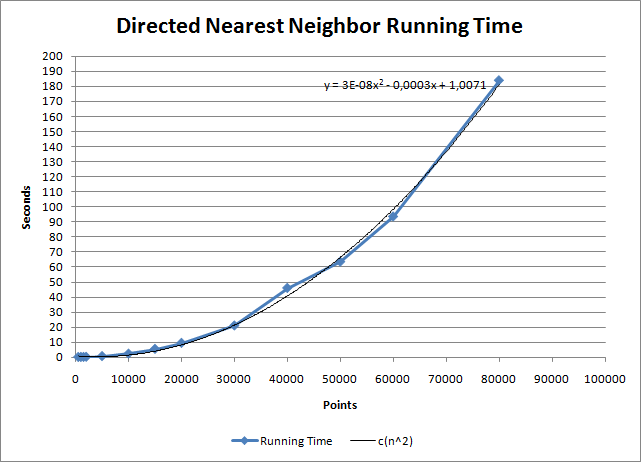
\includegraphics[scale = 0.6]{2DirectedNearestNeighbor/dnnRuntimeGraph.png}\\
        Figure 6: Graph of Directed Nearest Neighbor Running Time
        \end{center}

        \noindent When comparing the above running times to the ones from Nearest Neighbor, we observe this algorithm is indeed a little slower as we have shown in the running time analysis (\ref{sub:running_time_analysis}). However, when we introduce a trend line that derives a $n^2$ function from the results, we see that the algorithm is still $O(n^2)$.\\

        \subsection{Correct Output}
        After testing some of the test-cases, we noticed some of the previous algorithm's problems were now solved. The Flat test-case with 178 points was constructed correctly with the DirectedNearestNeighbor, but we also noticed test-cases still going wrong.
        This is due to that the algorithm still does not check for intersections when they are needed or not, another possibility is a non-optimal choice of the constant for determine the range. A clear example of this is the Spiral test-case. When we ran this with the above stated constant, we saw that because there were two points really close to each other (see red square in Figure 7), it does not choose the point after it correctly. This is because the next line to be drawn is much longer than $1.5$ times the small line between the previous two points.\\

        \begin{center}
          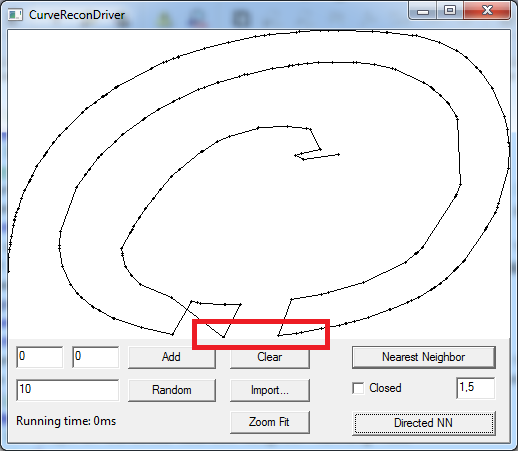
\includegraphics[scale = 0.6]{2DirectedNearestNeighbor/dnnSpiralgraph.png}\\
          Figure 7: Incorrect Spiral
        \end{center}

        \noindent Another thing we noticed was that the problem of lines going right through the graph still existed (and maybe even got worse). This is because, now that the algorithm is pickier, more points are left at the end. Since the algorithm wants to connect all points, it picks the ones left at the end.
        A solution for this could be checking for unused points at the end, and then try to insert these point in the correct place.\\

        \begin{center}
          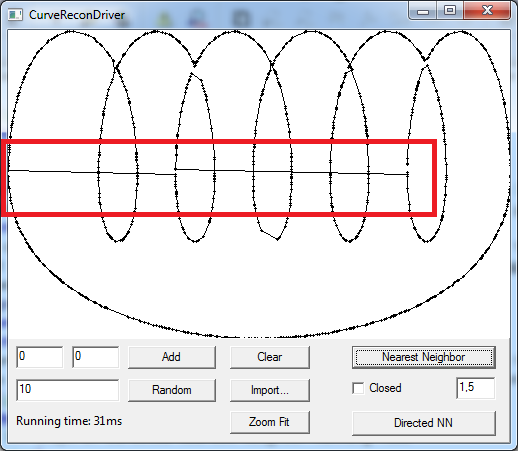
\includegraphics[scale = 0.6]{2DirectedNearestNeighbor/dnnSpringgraph.png}\\
          Figure 8: Incorrect Spring
        \end{center}

        \subsection{Conclusion from tests}
        When we look at several incorrect test-cases, we see that we need a better way of picking the range for Find-Points-In-Range. Also, we need to check for unused or incorrectly inserted points at the end. This is needed to make sure the points are inserted correctly and not just connected to each other at the end, messing up the curve. Another thing we could improve on is to look more carefully at the curve's direction, instead of just looking at angles to points in a certain range. Another improvement we should consider is to check for intersections at the end of reconstruction. 